\newcounter{alg:non-fifo:lines}
\begin{algo}[!ht]
\caption{SALSA implementation of SCPool: Data Structures.} 
\label{alg:non-fifo-ds}
\scriptsize
\begin{minipage}[t]{0.48\textwidth}
\begin{distribalgo}[1]
\smallskip

\INDENT {{\bf Chunk data structure}:}
	\STATE Task[CHUNK\_SIZE] tasks 
  \STATE int owner \comment {owner's consumer id}
\ENDINDENT

\INDENT {{\bf Node data structure}:}
  \STATE Chunk c; initially $\bot$
  \STATE int idx; initially -1
\ENDINDENT

\setcounter{alg:non-fifo:lines}{\value{ALC@line}} % store the line number
\end{distribalgo}
\end{minipage}%
%
\hfill
%
\begin{minipage}[t]{0.48\textwidth}
%
\begin{distribalgo}[1]
\setcounter{ALC@line}{\value{alg:non-fifo:lines}}
\smallskip

\INDENT {{\bf SALSA per consumer data structure}:}
  \STATE int consumerId
  \STATE List\tup{Node}[] chunkLists \comment {one list per producer + extra list for stealing (single-writer multi-reader)} 
  \STATE ChunkPool chunkPool \comment {the pool of spare chunks}
  \STATE Node currentNode, initially $\bot$ \comment {current node to work with} 
\ENDINDENT

\setcounter{alg:non-fifo:lines}{\value{ALC@line}}
\end{distribalgo}
\end{minipage}
\end{algo}


\begin{figure}[htb]
	\centering
	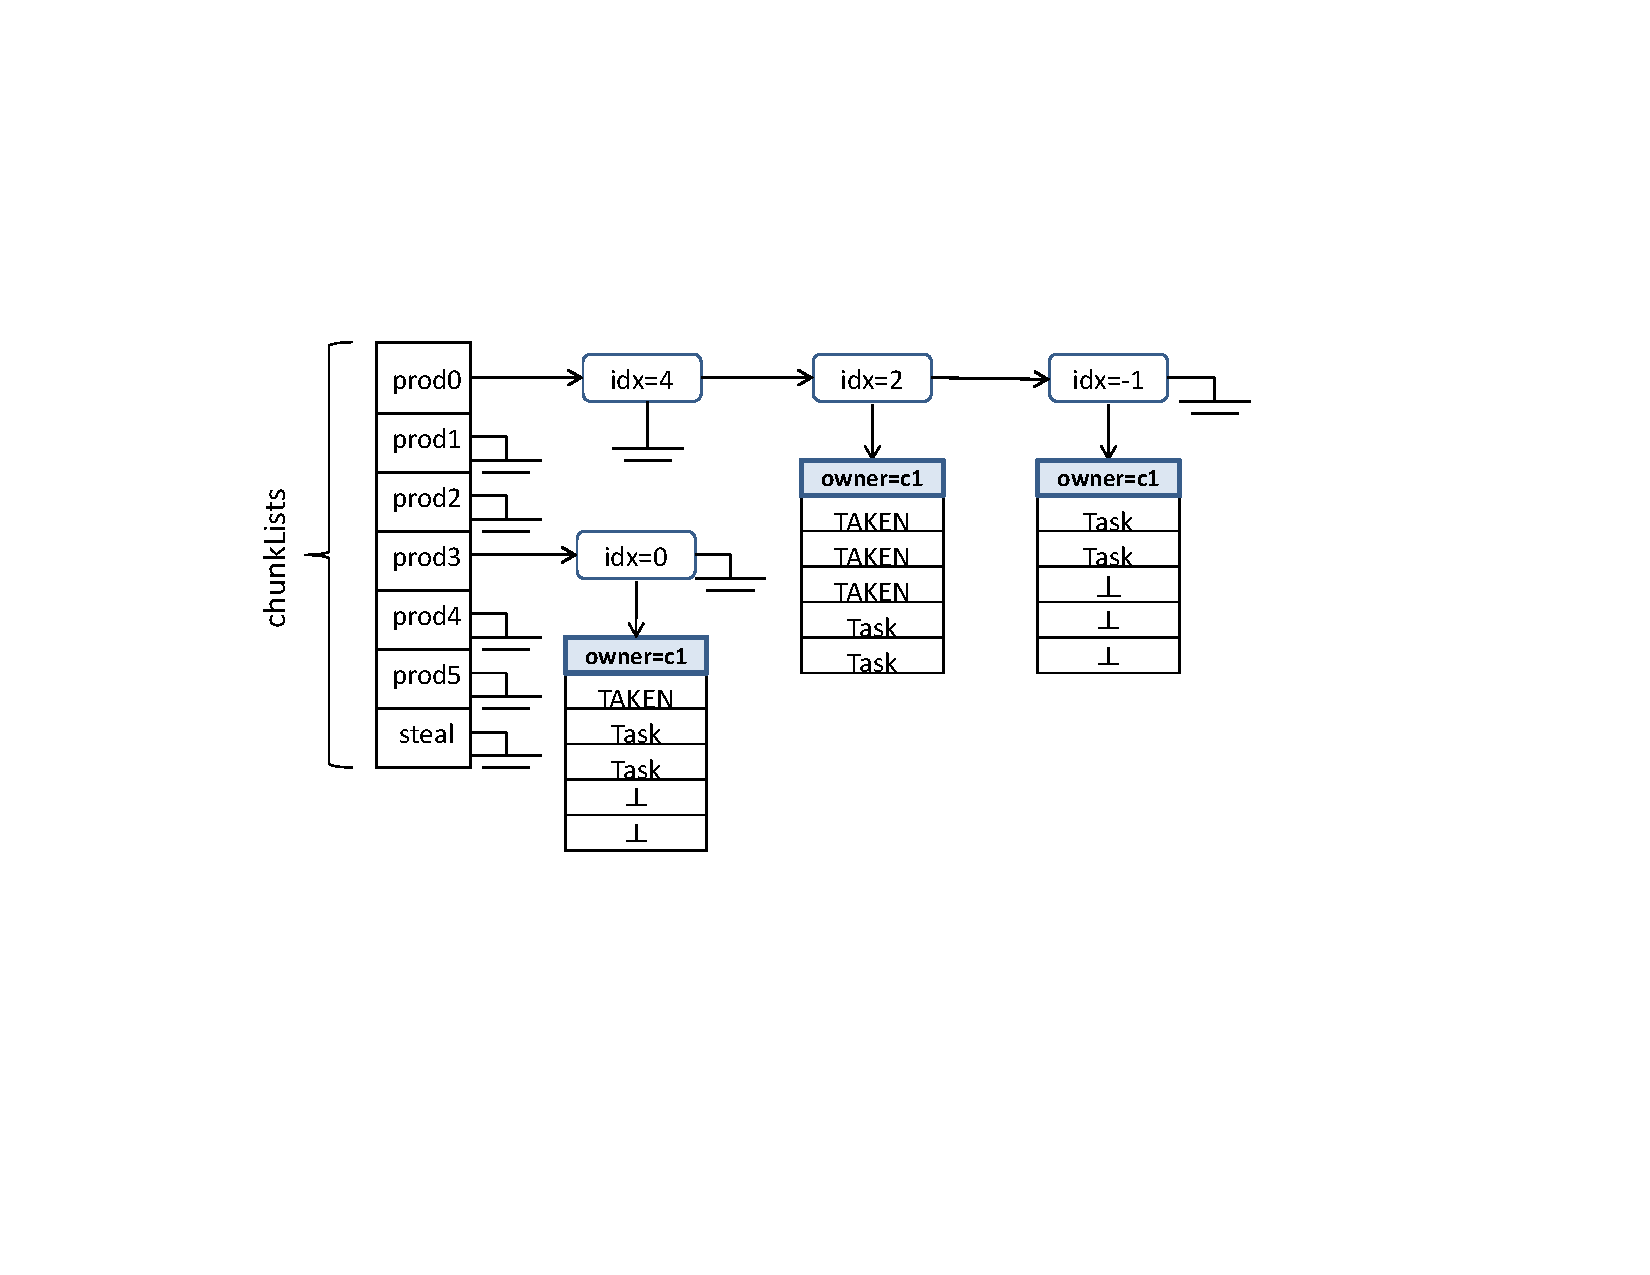
\includegraphics[height=0.3\textwidth]{figures/salsa-struct}
	\caption{
	    \footnotesize{Overview of the SALSA pool implementation. The tasks are kept in chunks, which are 
	    organized in per-producer lists (an additional list is reserved for stealing). Each list can be modified 
	    by the corresponding producer only. The only process that is allowed to retrieve tasks from a chunk is 
	    the owner of that chunk (defined by the ownership flag). Node index corresponds to the latest task taken from the chunk
	    or the task that is about to be taken by the current chunk owner. 
	    }}
	\label{fig:salsa-struct}
\end{figure}

As mentioned earlier, SALSA implements an API for a per-consumer pool, in this section the owner of the SALSA is consumer $c_i$ unless stated otherwise.
Its data structure is described in Algorithm~\ref{alg:non-fifo-ds} and depicted in Figure~\ref{fig:salsa-struct}. 
The tasks inserted to SALSA are kept in chunks, which are organized in per-producer chunk lists, i.e., only a single producer
can insert a task to a given chunk. Every chunk is owned by a single consumer whose id is kept at the \emph{owner} field of the chunk.
The owner is the only process that is allowed to take tasks from the chunk; if another process wants to take a task from the chunk, it should first steal the chunk and change its ownership. The owner of the chunk
residing at the pool of consumer $c_i$ is $c_i$ itself, unless that chunk is being stolen.

The per-producer chunk lists are kept in the array \emph{chunkLists}, where \emph{chunkLists[j]} keeps the chunks
with tasks inserted by producer $p_j$. 
In addition, the array has a special entry \emph{chunkLists[steal]}, which is reserved for the list of chunks stolen by $c_i$. 
The lists are single-writer lists: a list at \emph{chunkLists[j]} can be modified only by the producer $p_j$, the list at \emph{chunkLists[steal]} can be modified only by the owning consumer $c_i$. Since consumers can not modify the lists, nodes are lazily removed by the producers. Having a single writer allows us to implement the lists without synchronization primitives, similarly to the single-writer linked-list in~\cite{Michael:2004:HPS:987524.987595}.

Chunks are accessed via nodes of the chunk lists. In addition to the chunk pointer, each node keeps an index of the latest taken task. As we show in Section~\ref{alg-stealing}, this index plays a crucial role for chunk stealing. 
Safe memory reclamation is provided by using hazard pointers~\cite{Michael:2004:HPS:987524.987595} both for the nodes and the chunks.

The chunks in SALSA are kept in the per-consumer chunk pools, implemented using a lock-free Michael-Scott queue~\cite{Michael:1996:SFP:248052.248106}. 
These pools serve two purposes: 1) enable efficient memory reuse, 2) as we show in Section~\ref{alg-overview}, per-consumer chunk pools are good for load balancing. 

%owner last list, the only one to modify the list is the owner. Nodes are removed lazily: when a list
%owner sees a node that does not point to a chunk, this node is removed and reclaimed. When a
%producer wishes to add a new chunk to the list, he traverses the list, removing nodes without chunks
%while doing so, then he appends to the list a new node that points to the new chunk. Hazard
%pointers~\cite{Michael:2004:HPS:987524.987595} are used to manage the reclamation of nodes and
%chunks and solve the ABA problem.
%
%SALSA keeps an array of per-producer chunk lists; 
%an additional entry in the array is reserved for list of stolen chunks.  
%
%A producer inserts tasks to the chunks in its own list. 
%
%Every chunk has a single \emph{owner} process, which id is written in the owner field of that chunk. 
%The owner is the single consumer that is allowed to retrieve tasks
%from the chunk without synchronization. 
%
%
%
%In order to simplify stealing (see Section~\ref{alg-stealing}), chunks are accessed via \emph{nodes}
%Chunks are referred via the nodes, which keep 
%Each consumer pool is composed of chunk lists, each chunk for
%
% describe the structure of the SALSA implementation of a single-consumer pool.
%The structure is described in Algorithm~\ref{alg:non-fifo-ds} and Figure~\ref{fig:salsa-struct}
%
%The structure is composed of number of producers + 1 lists of nodes. The first lists corresponds to
%the producers, and the last list is used for stolen chunks. Each node has a pointer to a
%chunk and an index (idx), this indicates the index of the last task already taken or the index of
%a task which is about to be taken by the consumer, this field is used by a consumer to know what is
%the next available task in the chunk and it is also used when stealing chunks (see
%Section~\ref{alg-stealing}).
%Chunks are arrays of pointers to tasks. When there is no task in a cell it contains $\bot$, after
%the task was taken by a consumer, the cell will contain the special value \emph{TAKEN}. Each chunk
%has an owner which is the ID of the consumer that is currently working with that chunk. 
%
%The lists are single-writer multiple reader linked-lists, similar to the one shown
%in~\cite{Michael:2004:HPS:987524.987595}. Producer $i$ is owner of list $i$ and the consumer is the
%owner last list, the only one to modify the list is the owner. Nodes are removed lazily: when a list
%owner sees a node that does not point to a chunk, this node is removed and reclaimed. When a
%producer wishes to add a new chunk to the list, he traverses the list, removing nodes without chunks
%while doing so, then he appends to the list a new node that points to the new chunk. Hazard
%pointers~\cite{Michael:2004:HPS:987524.987595} are used to manage the reclamation of nodes and
%chunks and solve the ABA problem. 
%
%Each Consumer has a chunk pool, which is implemented using a
%lock-free queue~\cite{Michael:1996:SFP:248052.248106}. These pools are used to enable reuse of
%chunks, and also so producers can realize when a consumer is full and move to another consumer (see
%Section~\ref{alg-pools}).
